% !TeX root = ../main.tex
\documentclass[./../main.tex]{subfiles}

\begin{document}

Ứng dụng được triển khai tự động bằng Gitlab CI/CD thông qua các pipeline được config trên gitlab-ci.yml. Cụ thể, khi một commit được merge vào nhánh \code{master}, hệ thống CI sẽ tự động chạy toàn bộ unit test, build code ra phiên bản production và deploy code lên môi trường phù hợp.

Cách làm này không những tiết kiệm thời gian deploy, mà còn đảm bảo code hoạt động đúng như thiết kế trên môi trường production.

Với sản phẩm này, nhóm deploy frontend trên GitLab Pages, một trang hosting miễn phí.
Backend thì được build thành docker image và chạy trên một máy ảo của Google Cloud.
Ngoài ra, nhóm có sử dụng Docker để triển khai việc ảo hóa nên nhóm còn sử dụng thêm Nginx như một API Gateway đồng thời như
 là Reverse Proxy. Việc này sẽ đảm bảo cho hệ thống có khả năng scale up bằng cách tăng server API và che giấu đi việc cân
  bằng tải này. Đồng thời Nginx còn hỗ trợ việc logging và chống tấn công.

\begin{figure}[H]
	\centering
	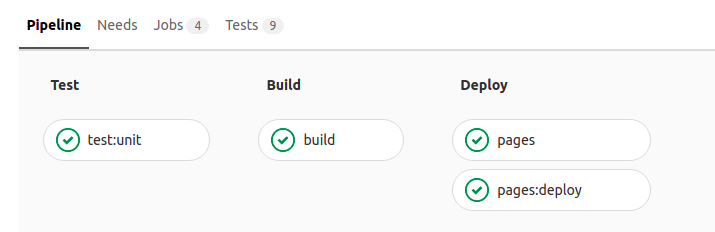
\includegraphics[width=\linewidth]{./images/pipeline_1.png}
	\caption{Pipeline cho Frontend}
\end{figure}

\begin{figure}[H]
	\centering
	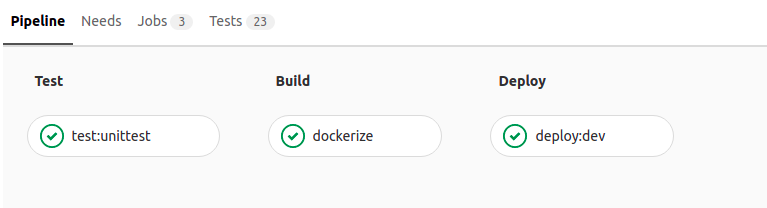
\includegraphics[width=\linewidth]{./images/pipeline_2.png}
	\caption{Pipeline cho backend}
\end{figure}

\end{document}